\PassOptionsToPackage{unicode}{hyperref}
\PassOptionsToPackage{hyphens}{url}
\PassOptionsToPackage{dvipsnames,svgnames,x11names}{xcolor}
\documentclass[
  letterpaper,
  DIV=11,
  numbers=noendperiod]{scrartcl}
\usepackage{xcolor}
\usepackage{amsmath,amssymb}
\setcounter{secnumdepth}{-\maxdimen} % remove section numbering
\usepackage{iftex}
\ifPDFTeX
  \usepackage[T1]{fontenc}
  \usepackage[utf8]{inputenc}
  \usepackage{textcomp} % provide euro and other symbols
\else % if luatex or xetex
  \usepackage{unicode-math} % this also loads fontspec
  \defaultfontfeatures{Scale=MatchLowercase}
  \defaultfontfeatures[\rmfamily]{Ligatures=TeX,Scale=1}
\fi
\usepackage{lmodern}
\ifPDFTeX\else
\fi
\IfFileExists{upquote.sty}{\usepackage{upquote}}{}
\IfFileExists{microtype.sty}{% use microtype if available
  \usepackage[]{microtype}
  \UseMicrotypeSet[protrusion]{basicmath} % disable protrusion for tt fonts
}{}
\makeatletter
\@ifundefined{KOMAClassName}{% if non-KOMA class
  \IfFileExists{parskip.sty}{%
    \usepackage{parskip}
  }{% else
    \setlength{\parindent}{0pt}
    \setlength{\parskip}{6pt plus 2pt minus 1pt}}
}{% if KOMA class
  \KOMAoptions{parskip=half}}
\makeatother
\makeatletter
\ifx\paragraph\undefined\else
  \let\oldparagraph\paragraph
  \renewcommand{\paragraph}{
    \@ifstar
      \xxxParagraphStar
      \xxxParagraphNoStar
  }
  \newcommand{\xxxParagraphStar}[1]{\oldparagraph*{#1}\mbox{}}
  \newcommand{\xxxParagraphNoStar}[1]{\oldparagraph{#1}\mbox{}}
\fi
\ifx\subparagraph\undefined\else
  \let\oldsubparagraph\subparagraph
  \renewcommand{\subparagraph}{
    \@ifstar
      \xxxSubParagraphStar
      \xxxSubParagraphNoStar
  }
  \newcommand{\xxxSubParagraphStar}[1]{\oldsubparagraph*{#1}\mbox{}}
  \newcommand{\xxxSubParagraphNoStar}[1]{\oldsubparagraph{#1}\mbox{}}
\fi
\makeatother

\usepackage{longtable,booktabs,array}
\newcounter{none} % for unnumbered tables
\usepackage{calc} % for calculating minipage widths
\usepackage{etoolbox}
\makeatletter
\patchcmd\longtable{\par}{\if@noskipsec\mbox{}\fi\par}{}{}
\makeatother
\IfFileExists{footnotehyper.sty}{\usepackage{footnotehyper}}{\usepackage{footnote}}
\makesavenoteenv{longtable}
\usepackage{graphicx}
\makeatletter
\newsavebox\pandoc@box
\newcommand*\pandocbounded[1]{% scales image to fit in text height/width
  \sbox\pandoc@box{#1}%
  \Gscale@div\@tempa{\textheight}{\dimexpr\ht\pandoc@box+\dp\pandoc@box\relax}%
  \Gscale@div\@tempb{\linewidth}{\wd\pandoc@box}%
  \ifdim\@tempb\p@<\@tempa\p@\let\@tempa\@tempb\fi% select the smaller of both
  \ifdim\@tempa\p@<\p@\scalebox{\@tempa}{\usebox\pandoc@box}%
  \else\usebox{\pandoc@box}%
  \fi%
}
\def\fps@figure{htbp}
\makeatother

\setlength{\emergencystretch}{3em} % prevent overfull lines

\providecommand{\tightlist}{%
  \setlength{\itemsep}{0pt}\setlength{\parskip}{0pt}}

\KOMAoption{captions}{tableheading}
\makeatletter
\@ifpackageloaded{caption}{}{\usepackage{caption}}
\AtBeginDocument{%
\ifdefined\contentsname
  \renewcommand*\contentsname{Table of contents}
\else
  \newcommand\contentsname{Table of contents}
\fi
\ifdefined\listfigurename
  \renewcommand*\listfigurename{List of Figures}
\else
  \newcommand\listfigurename{List of Figures}
\fi
\ifdefined\listtablename
  \renewcommand*\listtablename{List of Tables}
\else
  \newcommand\listtablename{List of Tables}
\fi
\ifdefined\figurename
  \renewcommand*\figurename{Figure}
\else
  \newcommand\figurename{Figure}
\fi
\ifdefined\tablename
  \renewcommand*\tablename{Table}
\else
  \newcommand\tablename{Table}
\fi
}
\@ifpackageloaded{float}{}{\usepackage{float}}
\floatstyle{ruled}
\@ifundefined{c@chapter}{\newfloat{codelisting}{h}{lop}}{\newfloat{codelisting}{h}{lop}[chapter]}
\floatname{codelisting}{Listing}
\newcommand*\listoflistings{\listof{codelisting}{List of Listings}}
\makeatother
\makeatletter
\makeatother
\makeatletter
\@ifpackageloaded{caption}{}{\usepackage{caption}}
\@ifpackageloaded{subcaption}{}{\usepackage{subcaption}}
\makeatother
\usepackage{bookmark}
\IfFileExists{xurl.sty}{\usepackage{xurl}}{} % add URL line breaks if available
\urlstyle{same}
\hypersetup{
  pdftitle={Problem Set 7: Inferring methyltransferase binding rates},
  pdfauthor={Jun Allard},
  colorlinks=true,
  linkcolor={blue},
  filecolor={Maroon},
  citecolor={Blue},
  urlcolor={Blue},
  pdfcreator={LaTeX via pandoc}}

\ifXeTeX
\special{pdf:trailerid [ <d14882e4e52005a9bdf713d5546c14f9> <d14882e4e52005a9bdf713d5546c14f9> ]}
\fi
\ifPDFTeX
\pdftrailerid{}
\pdftrailer{/ID [ <d14882e4e52005a9bdf713d5546c14f9> <d14882e4e52005a9bdf713d5546c14f9> ]}
\fi
\ifLuaTeX
\pdfvariable trailerid {[ <d14882e4e52005a9bdf713d5546c14f9> <d14882e4e52005a9bdf713d5546c14f9> ]}
\fi

\title{Problem Set 7: Inferring methyltransferase binding rates}
\usepackage{etoolbox}
\makeatletter
\providecommand{\subtitle}[1]{% add subtitle to \maketitle
  \apptocmd{\@title}{\par {\large #1 \par}}{}{}
}
\makeatother
\subtitle{Physics 230A/146A --- Biological Physics}
\author{Jun Allard}
\date{}
\begin{document}
\maketitle


Suppose a system can transition between two states, State 1 and State 2, with transition rates \(k_{1\rightarrow 2}\) and \(k_{2\rightarrow 1}\).
If transitions are driven by thermal fluctuations, then these transition rates must obey

\begin{equation}\protect\phantomsection\label{eq-detailed-balance-2}{
\frac{k_{1\rightarrow 2}}{k_{2\rightarrow 1}} = e^{-(E_2-E_1)/k_BT} = e^{-(\Delta E_{12})/k_BT}
}\end{equation}

where \(E_1\) and \(E_2\) are the energies of those two states.

If a system can transition between 3 states, State A, State B and State C, and transitions are driven by thermal fluctuations, then it follows from Equation~\ref{eq-detailed-balance-2} that

\begin{equation}\protect\phantomsection\label{eq-detailed-balance-3}{
\frac{k_{A\rightarrow C}}{k_{C\rightarrow A}} = \frac{k_{A\rightarrow B}}{k_{B\rightarrow A}} \cdot \frac{k_{B\rightarrow C}}{k_{C\rightarrow B}}.
}\end{equation}

This means that, to find all 6 transition rates, an experimentalist would only need to measure 5 rates.
The sixth (whichever it is) could then be computed from Equation~\ref{eq-detailed-balance-3}.

\subsection{A.}\label{a.}

A methyltransferase called DNMT loads a methyl group (from S-Adenosyl methionine), binds to DNA, and attaches the methyl to the DNA.
This is a form of epigenetic regulation that plays a role in cell fate determination\footnote{L. Busto-Moner, J. Morival, H. Ren, A. Fahim, Z. Reitz, T. L. Downing, E. L. Read. Stochastic modeling reveals kinetic heterogeneity in post-replication DNA methylation. PLOS Computational Biology (2020).}
Thus, it can exist in 4 states: bound or unbound to DNA, carrying or not carrying a methyl.

\begin{center}
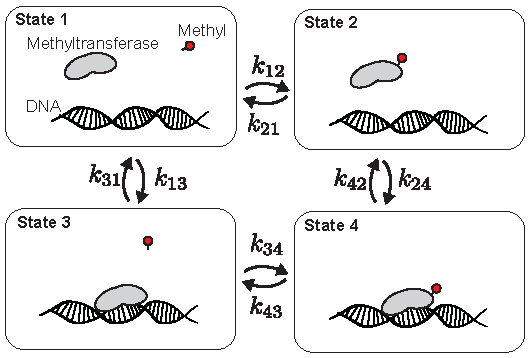
\includegraphics[width=10cm,height=\textheight,keepaspectratio]{fig_methyltransferase-rates.pdf}
\end{center}

Suppose that only one binding/unbinding event or loading/unloading event can occur at a time, in which case only the 8 transitions shown in the diagram are allowed (i.e., you may assume the 4 ``diagonal'' transitions have zero rate).

\begin{enumerate}
\def\labelenumi{\roman{enumi}.}
\tightlist
\item
  The rate constraint equation above for 3-states, Equation~\ref{eq-detailed-balance-3}, is a constraint purely involving rates (\(k\)'s) and no state energies or probabilities.
  For the 4-state system, find all constraints on the rates that only involve rates (\(k\), no state energies or probabilities) that are produced by the Principle of Detailed Balance.
\item
  How many are there? And therefore, how many independent rates must the experimentalist measure?
\end{enumerate}

\subsection{B.}\label{b.}

Suppose a system can transition between \(N\) states, \(i=1..N\).
There are, in general, \(N\cdot(N-1)\) transition rates.
If the system obeys Detailed Balance, how many constraints are there?
And therefore, how many independent rates must an experimentalist measure?
Note that in Part A, we assumed that there were 4 states and only 8 non-zero transitions, whereas in general, a 4-state system has 12 transitions.




\end{document}
